%& /Users/ziky/.cache/org-persist/5d/395a48-6702-4626-bf4d-f48ac73e8a5b-832ed4017c79fd5b5d686e66a4a447c3
% Created 2025-10-27 Mon 12:18
% Intended LaTeX compiler: pdflatex
\documentclass[11pt]{article}
\usepackage[utf8]{inputenc}
\usepackage[T1]{fontenc}
\usepackage{amsmath}
\usepackage{amssymb}
\usepackage{capt-of}
\usepackage{hyperref}
\setlength{\abovedisplayskip}{0pt}
\setlength{\belowdisplayskip}{0pt}
\usepackage[a4paper, margin=1in]{geometry}

%% ox-latex features:
%   !announce-start, !guess-pollyglossia, !guess-babel, !guess-inputenc,
%   caption, maths, image, !announce-end.

\usepackage{capt-of}

\usepackage{amsmath}
\usepackage{amssymb}

\usepackage{graphicx}

%% end ox-latex features


% end precompiled preamble
\ifcsname endofdump\endcsname\endofdump\fi

\author{Ziky Zhang}
\date{\today}
\title{Worksheet \#8}
\hypersetup{
 pdfauthor={Ziky Zhang},
 pdftitle={Worksheet \#8},
 pdfkeywords={},
 pdfsubject={},
 pdfcreator={},
 pdflang={English}}
\begin{document}

\maketitle
\begin{enumerate}
\item A long wire with a circular cross-section (\(1.9 \mathrm{mm}\) diameter) carries a current of \(8.0 \mathrm{mA}\). The wire is made of a hypothetical material having the following properties:
\begin{itemize}
\item resistivity = \(5.6 \times 10^{-8} \ \Omega \mathrm{m}\)
\item density = \(21.4 \ \mathrm{g} / \mathrm{cm}^3\)
\item atomic mass = \(138.9055 \ \mathrm{g} / \mathrm{mole}\)
\item atomic number = \(59\)
\end{itemize}
\begin{enumerate}
\item Calculate the electric field inside the wire.
The drift velocity is measured (via the Hall Effect, to be discussed in Chapter 28) to be \(9.50 \times 10^{-8} \ \mathrm{m} / \mathrm{s}\).
\item Calculate the number density of conduction electrons in the hypothetical material.
\item On average, how many conduction electrons are available per atom?
\end{enumerate}
\item The filament of a certain light bulb is made of tungsten and has a length of \(0.48 \mathrm{m}\) and a circular cross-section with a diameter of \(0.062 \mathrm{mm}\).
\begin{enumerate}
\item Calculate the resistance of the filament at room temperature.
\item A \(4.0 \mathrm{V}\) voltage applied to the filament results in a \(0.078 \mathrm{A}\) current. Determine the temperature of the filament under these conditions.
\end{enumerate}
\item Three batteries are connected in the circuit given below.
\begin{figure}[htbp]
\centering
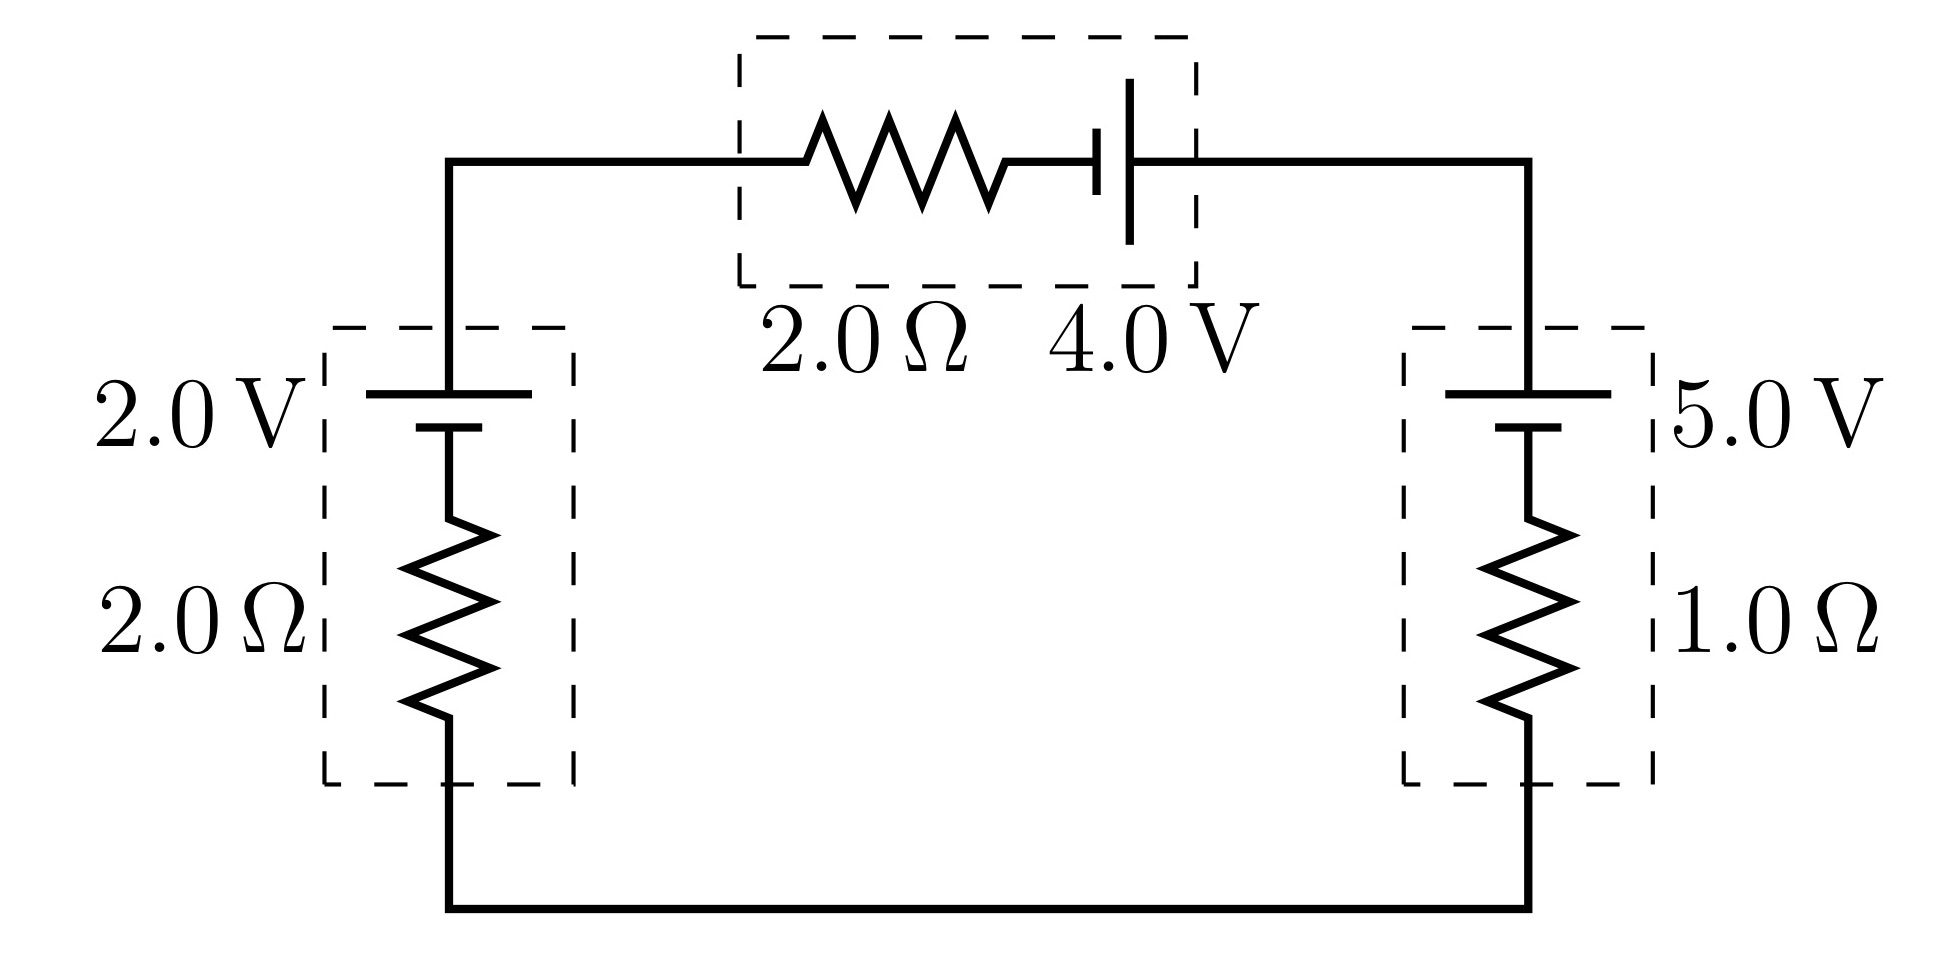
\includegraphics[height=3cm]{./img/8.1.jpg}
\caption{\label{fig:orga4c70be}Single-loop circuit with three batteries}
\end{figure}
\begin{enumerate}
\item Determine the current through the circuit (be sure to indicate its direction).
\item Calculate the voltage across each battery.
\item Determine the rate in which chemical energy is either used or restored in each battery.
\end{enumerate}
\end{enumerate}

\newpage
1.(a)
\begin{align*}
\overrightarrow{E} &= \rho J \\
  &= \rho \frac{I}{A} \\
  &= 5.6 \times 10^{-8} \ \Omega \mathrm{m} \frac{0.008 \mathrm{A}}{\pi (\frac{1}{2} \cdot 0.0019 \mathrm{m})^{2}} \\
  &= 5.6 \times 10^{-8} \ \Omega \mathrm{m} \frac{8 \times 10^{-3} \mathrm{A}}{\pi (9.025 \times 20^{-7} \ \mathrm{m}^{2})} \\
  &= 5.6 \times 10^{-8} \ \Omega \mathrm{m} \frac{8 \times 10^{-3} \mathrm{A}}{2.86 \times 10^{-6} \mathrm{m}^{2}} \\
  &= 5.6 \times 10^{-8} \ \Omega \cdot 2.80 \times 10^{3} \frac{\mathrm{A}}{\mathrm{m}} \\
  &= 1.57 \times 10^{-4} \ \Omega \frac{\mathrm{A}}{\mathrm{m}} \\
\end{align*}

1.(b)
\begin{align*}
J &= ne v_d \\
n_{\mathrm{electron,\  cond}} &= \frac{J}{e v_d} \\
  &= \frac{2.80 \times 10^3 \frac{A}{\mathrm{m}^2}}{1.602 \times 10^{-19} \mathrm{C} \cdot 9.5 \times 10^{-8} \frac{\mathrm{m}}{\mathrm{s}}} \\
  &= \frac{2.80 \times 10^{30} \mathrm{m}^2}{15.219 \mathrm{m}} \\
  &= 1.840 \times 10^{29} \mathrm{m}^{-3}
\end{align*}

1.(c)
\begin{align*}
\begin{aligned}[t]
\text{Variables: }
\rho_{\mathrm{den}} &= 21.4 \ \mathrm{g}/\mathrm{cm}^{3} \\
m &= 138.9055 \ \mathrm{g} / \mathrm{mole} \\
N_A &= 6.022 \times 10^{23} \mathrm{atoms}/\mathrm{mole} \\
\end{aligned}
\qquad
\begin{aligned}[t]
n_{\mathrm{atom}} &= \frac{p_{den} N_A}{m} \\
  &= \frac{21.4 \tfrac{\mathrm{g}}{\mathrm{cm}^{3}} \cdot 6.022 \times 10^{23} \frac{\mathrm{atoms}}{\mathrm{mole}}}{138.9055 \tfrac{\mathrm{g}}{\mathrm{mole}}} \\
  &= \frac{21.4 \times 10^{7} \ \mathrm{g}}{\mathrm{m}^{3}} \cdot \frac{6.022 \times 10^{23} \mathrm{atoms}}{\mathrm{mole}} \cdot \frac{\mathrm{mole}}{138.9055 \ \mathrm{g}} \\
  &= \frac{128.8708 \times 10^{31}}{138.9055 \ \mathrm{m}^{3}} \\
  &= 9.278 \times 10^{28} \mathrm{m}^{-3}
\end{aligned}
\end{align*}
\begin{align*}
\frac{n_{\mathrm{electron, \ cond}}}{n_{\mathrm{atom}}} &= \frac{1.840 \times 10^{29} \mathrm{m}^{-3}}{9.278 \times 10^{28} \mathrm{m}^{-3}} \\
  &\approx 1.983186031 \approx 2 \frac{\mathrm{electrons}}{\mathrm{atom}}
\end{align*}

\newpage
2.(a)
\begin{align*}
\begin{aligned}[t]
\text{Variables: }
\rho &= 5.25 \times 10^{-8} \Omega \mathrm{m}\\
L &= .48 \mathrm{m} \\
d &= .062 \mathrm{mm} = .000062 \mathrm{m}
\end{aligned}
\qquad
\begin{aligned}[t]
R &= \rho \frac{L}{A} \\
  &= 5.25 \times 10^{-8} \Omega \mathrm{m} \cdot \frac{.48 \mathrm{m}}{\pi (d/2)^2} \\
  &= 5.25 \times 10^{-8} \Omega \mathrm{m} \cdot \frac{.48 \mathrm{m}}{3.019 \times 10^{-9} \mathrm{m}^2} \\
  &= \frac{2.52 \times 10^{-8} \Omega \mathrm{m}^2}{3.019 \times 10^{-9} \mathrm{m}^2} \\
  &= 8.347 \Omega
\end{aligned}
\end{align*}

2.(b)
\begin{align*}
\begin{aligned}[t]
\text{Variables: }
V &= 4.0 \mathrm{V} \\
I &= 0.078 \mathrm{A} \\
\rho_0 &= 5.25 \times 10^{-8} \Omega \mathrm{m} \\
T_0 &= 293 \mathrm{K} \\
\alpha &= 4.5 \times 10^{-3} \mathrm{K}^{-1} \\
\end{aligned}
\qquad
\begin{aligned}[t]
\rho - \rho_0 &= \rho_0 \alpha (T - T_0) \\
\rho - \rho_0 &= \rho_0 \alpha T - \rho_0 \alpha T_0 \\
\rho_0 \alpha T &= R \frac{A}{L} - \rho_0 + \rho_0 \alpha T_0 \\
T &= \frac{R \frac{A}{L} - \rho_0 }{\rho_0 \alpha} + T_0 \\
  &= \frac{32.255 \times 10^{-8} \Omega \mathrm{m} - 5.25 \times 10^{-8} \Omega \mathrm{m}}{5.25 \times 10^{-8} \Omega \mathrm{m} \cdot 4.5 \times 10^{-3} \mathrm{K}^{-1}} + 293 \mathrm{K} \\
  &= \frac{27.005 \times 10^{-8} \Omega \mathrm{m}}{5.25 \times 10^{-8} \Omega \mathrm{m} \cdot 4.5 \times 10^{-3}} \mathrm{K} + 293 \mathrm{K} \\
  &= 1143.1 \mathrm{K} + 293 \mathrm{K} \\
  &= 1436.1 \mathrm{K}
\end{aligned}
\end{align*}

3.(a)
\begin{align*}
I &= \frac{\mathcal{E}_{\mathrm{left}} + \mathcal{E}_{\mathrm{top}} - \mathcal{E}_{\mathrm{right}}}{r_{\mathrm{left}} + r_{\mathrm{top}} + r_{\mathrm{right}}} \\
  &= \frac{1.0 \mathrm{V}}{5 \Omega} \\
  &= .2 \mathrm{A, \ clockwise}
\end{align*}

3.(b)
\begin{align*}
\begin{aligned}[t]
\Delta V_{\mathrm{left}} &= - Ir_{\mathrm{left}} + \mathcal{E}_{\mathrm{left}} \\
  &= - .2 \mathrm{A} \cdot 2.0 \Omega + 2.0 \mathrm{V} \\
  &= 1.6 \mathrm{V}
\end{aligned}
\quad
\begin{aligned}[t]
\Delta V_{\mathrm{top}} &= - Ir_{\mathrm{top}} + \mathcal{E}_{\mathrm{top}} \\
  &= - .2 \mathrm{A} \cdot 2.0 \Omega + 4.0 \mathrm{V} \\
  &= 3.6 \mathrm{V}
\end{aligned}
\quad
\begin{aligned}[t]
\Delta V_{\mathrm{right}} &= - Ir_{\mathrm{right}} - \mathcal{E}_{\mathrm{rihgt}} \\
  &= - .2 \mathrm{A} \cdot 1.0 \Omega - 5.0 \mathrm{V} \\
  &= -5.2 \mathrm{V}
\end{aligned}
\end{align*}

3.(c)
\begin{align*}
\begin{aligned}[t]
P_{left} &= - V_{left} I \\
  &= - 1.6 \mathrm{V} \cdot .2 \mathrm{A} \\
  &= - 0.32 \mathrm{W}
\end{aligned}
\quad
\begin{aligned}[t]
P_{top} &= - V_{top} I \\
  &= - 3.6 \mathrm{V} \cdot .2 \mathrm{A} \\
  &= - 0.72 \mathrm{W}
\end{aligned}
\quad
\begin{aligned}[t]
P_{right} &= - V_{right} I \\
  &=  5.2 \mathrm{V} \cdot .2 \mathrm{A} \\
  &=  1.04 \mathrm{W}
\end{aligned}
\quad
\end{align*}
\end{document}
